 
To determine the efficiency of the double lepton triggers, we derive the efficiency of the requirements imposed on each leg separately.
This requires a modification to the tag and probe method described above in some cases.
If the trigger objects are saved by the HLT before the requirement that there be two valid objects then
we can check each leg independently of the other using the usual tag and probe method.
If the trigger objects are saved after the requirement that there are two valid objects, then there is 
a 100\% correlation between the decision we can probe on each lepton.
This means that we must pick exactly one tag candidate for each event a priori, which we do 
randomly. 
If the randomly selected tag candidate meets the tight requirements then we are free to 
probe the other lepton.

Having measured the per lepton trigger trigger efficiency,
it is necessary to compute the expected efficiency for dilepton events to pass the trigger.
This is done by taking into account the $p_{T}$ and $\eta$ distributions
of both leptons in the signal sample.

\subsubsection{Electron triggers}
%%%%%% double
The double electron trigger requires the higher $p_T$ leg to be seeded at Level-1.
The per electron efficiency for both the seeded leg is shown in 
Figure \ref{fig:Ele17Ele8TriggerEfficiencySeededLeg} as a function of $p_{T}$ and $\eta$, 
and the unseeded leg is shown in Figure \ref{fig:Ele17Ele8TriggerEfficiencyUnseededLeg}.
The results are summarised in Table \ref{tab:eff_double_ele}. 

\begin{figure}[!ht]
\begin{center}
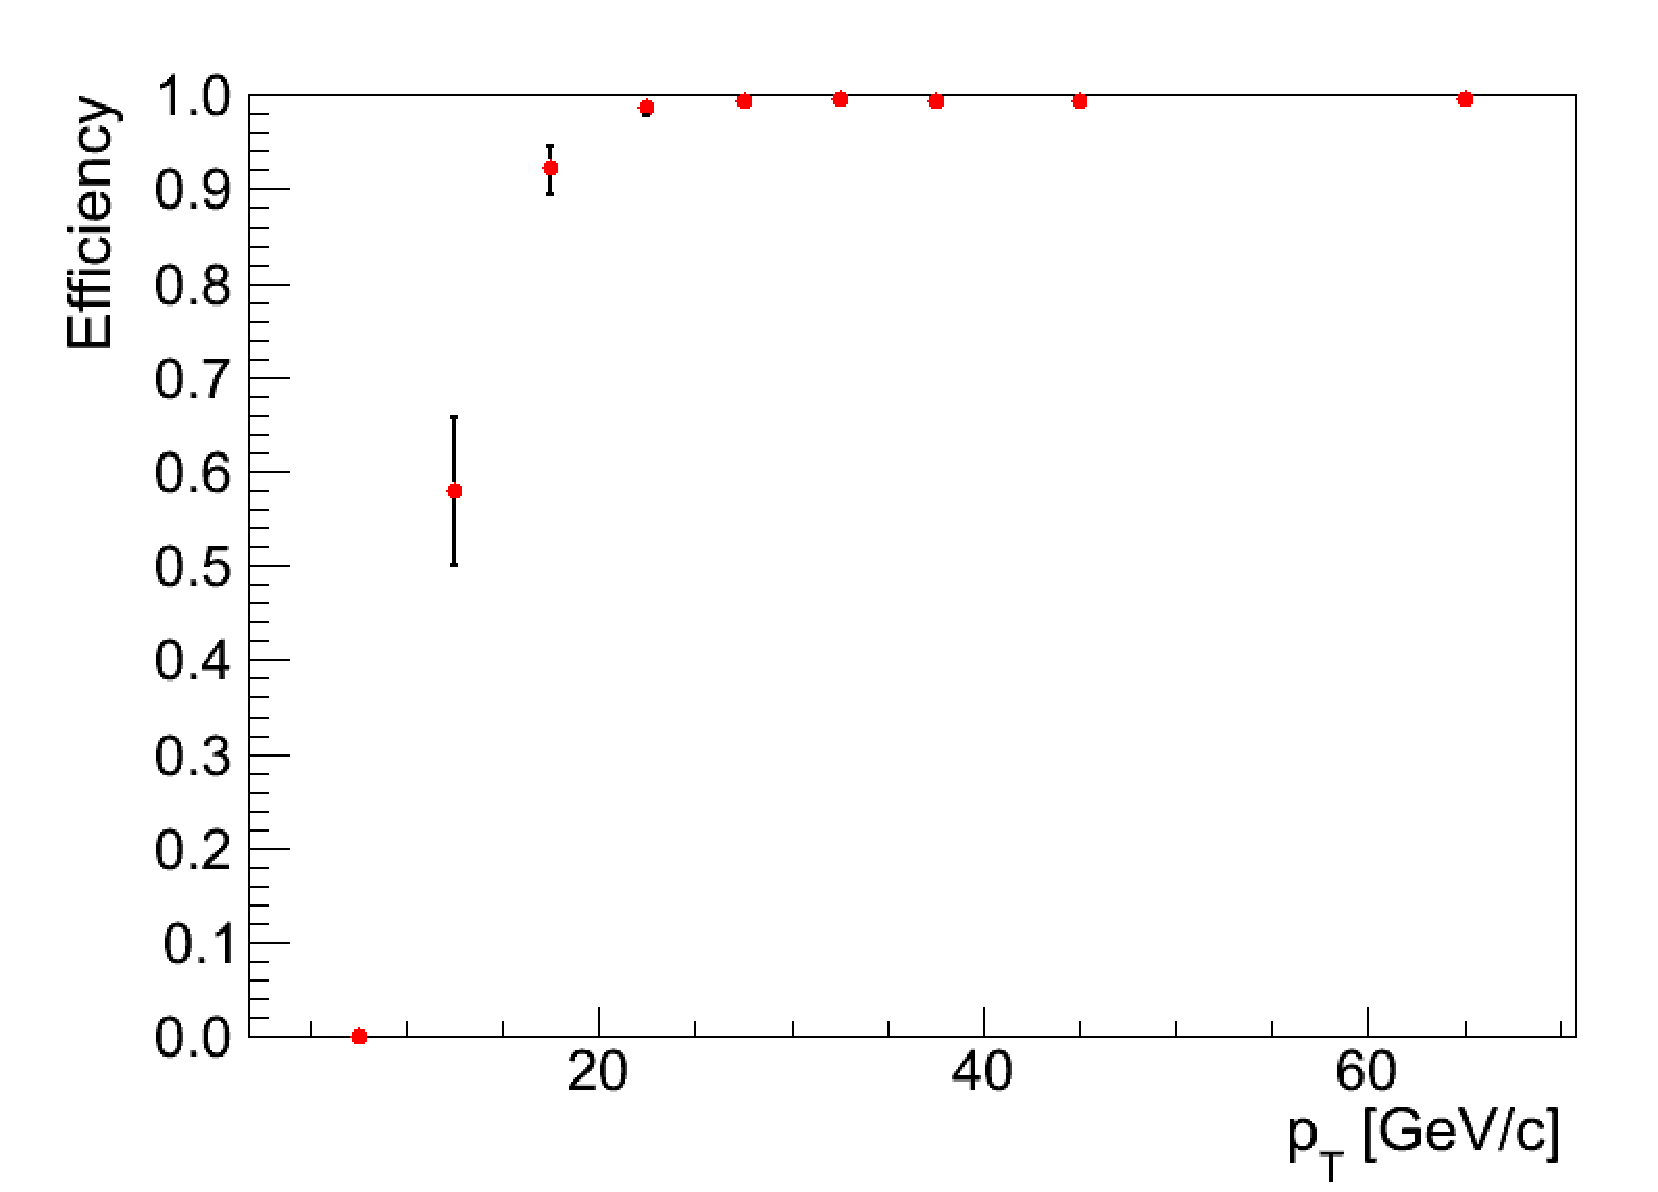
\includegraphics[width=0.48\textwidth]{figures/ElectronTriggerEffVsPt_Ele17Ele8WithL1Seed.pdf}
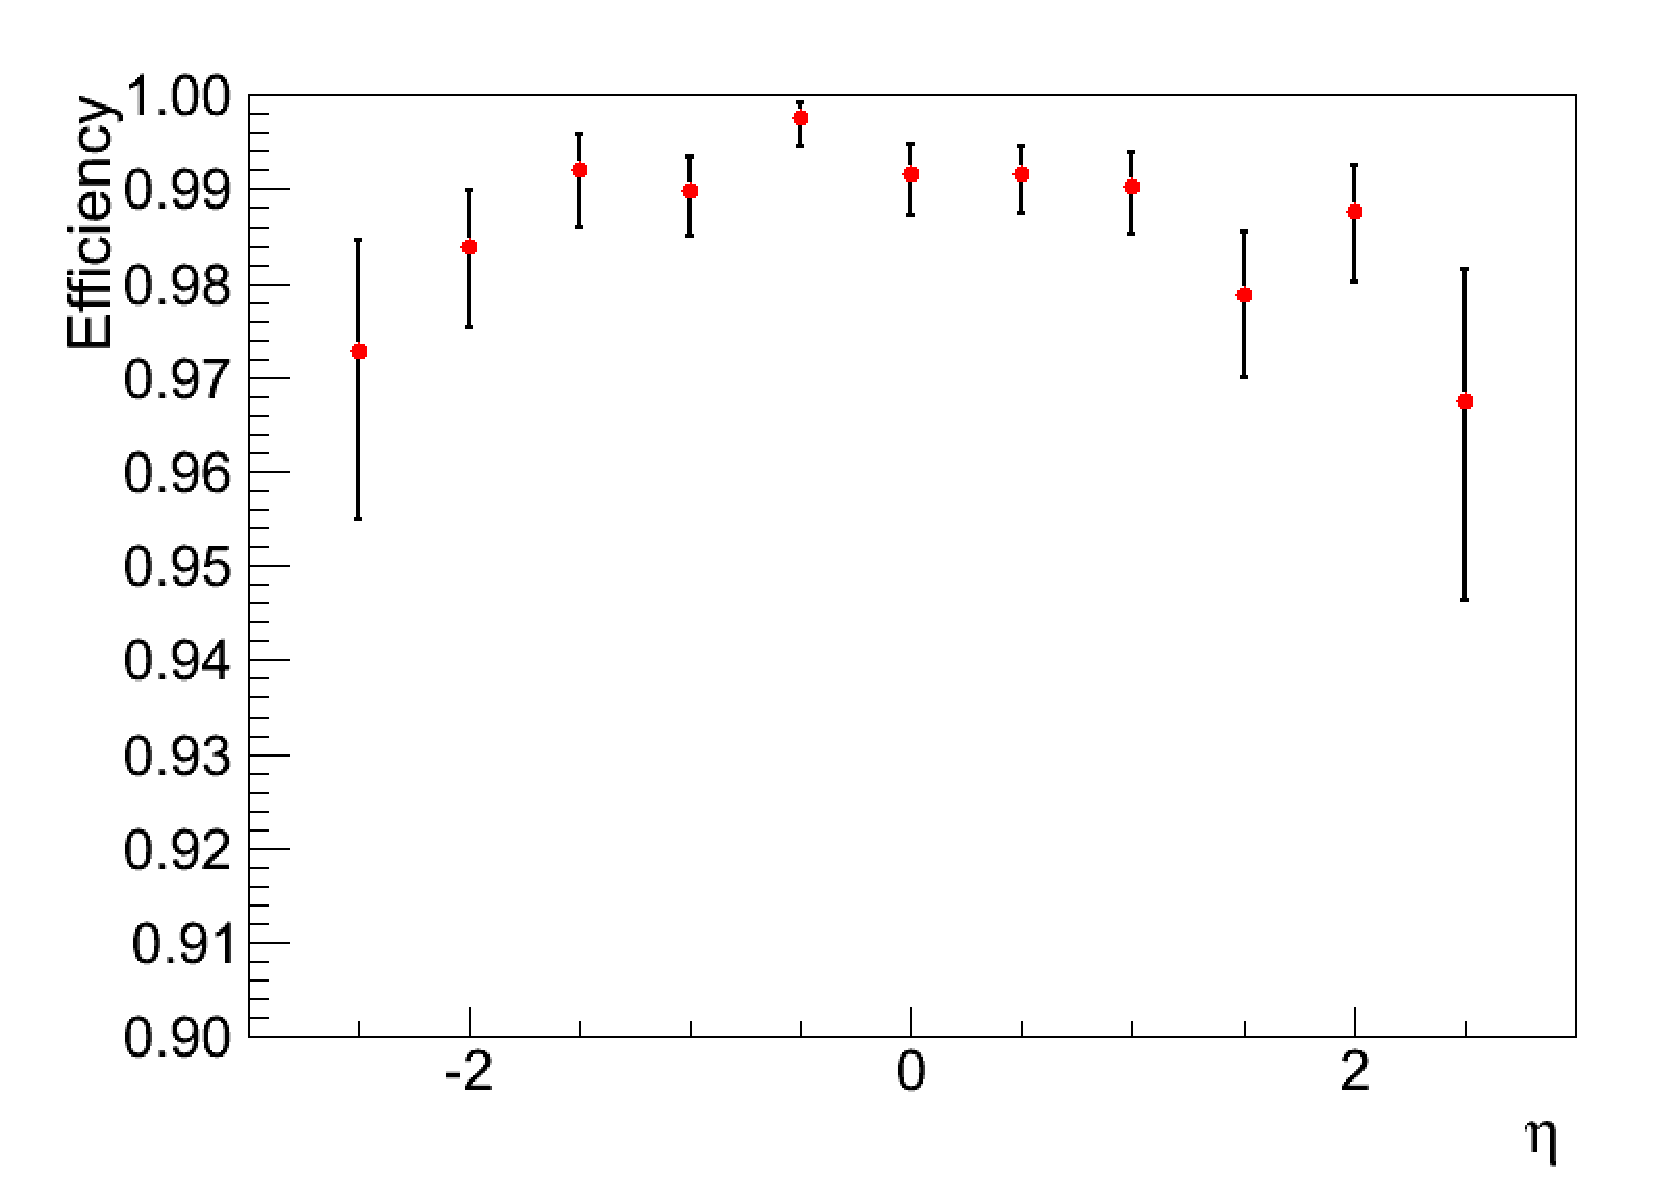
\includegraphics[width=0.48\textwidth]{figures/ElectronTriggerEffVsEta_Ele17Ele8WithL1Seed.pdf}
\end{center}
\caption{Efficiency for the L1 seeded leg of the double electron trigger as a function of $p_{T}$ (a) and $\eta$ (b).}
\label{fig:Ele17Ele8TriggerEfficiencySeededLeg}
\end{figure} 
\begin{figure}[!ht]
\begin{center}
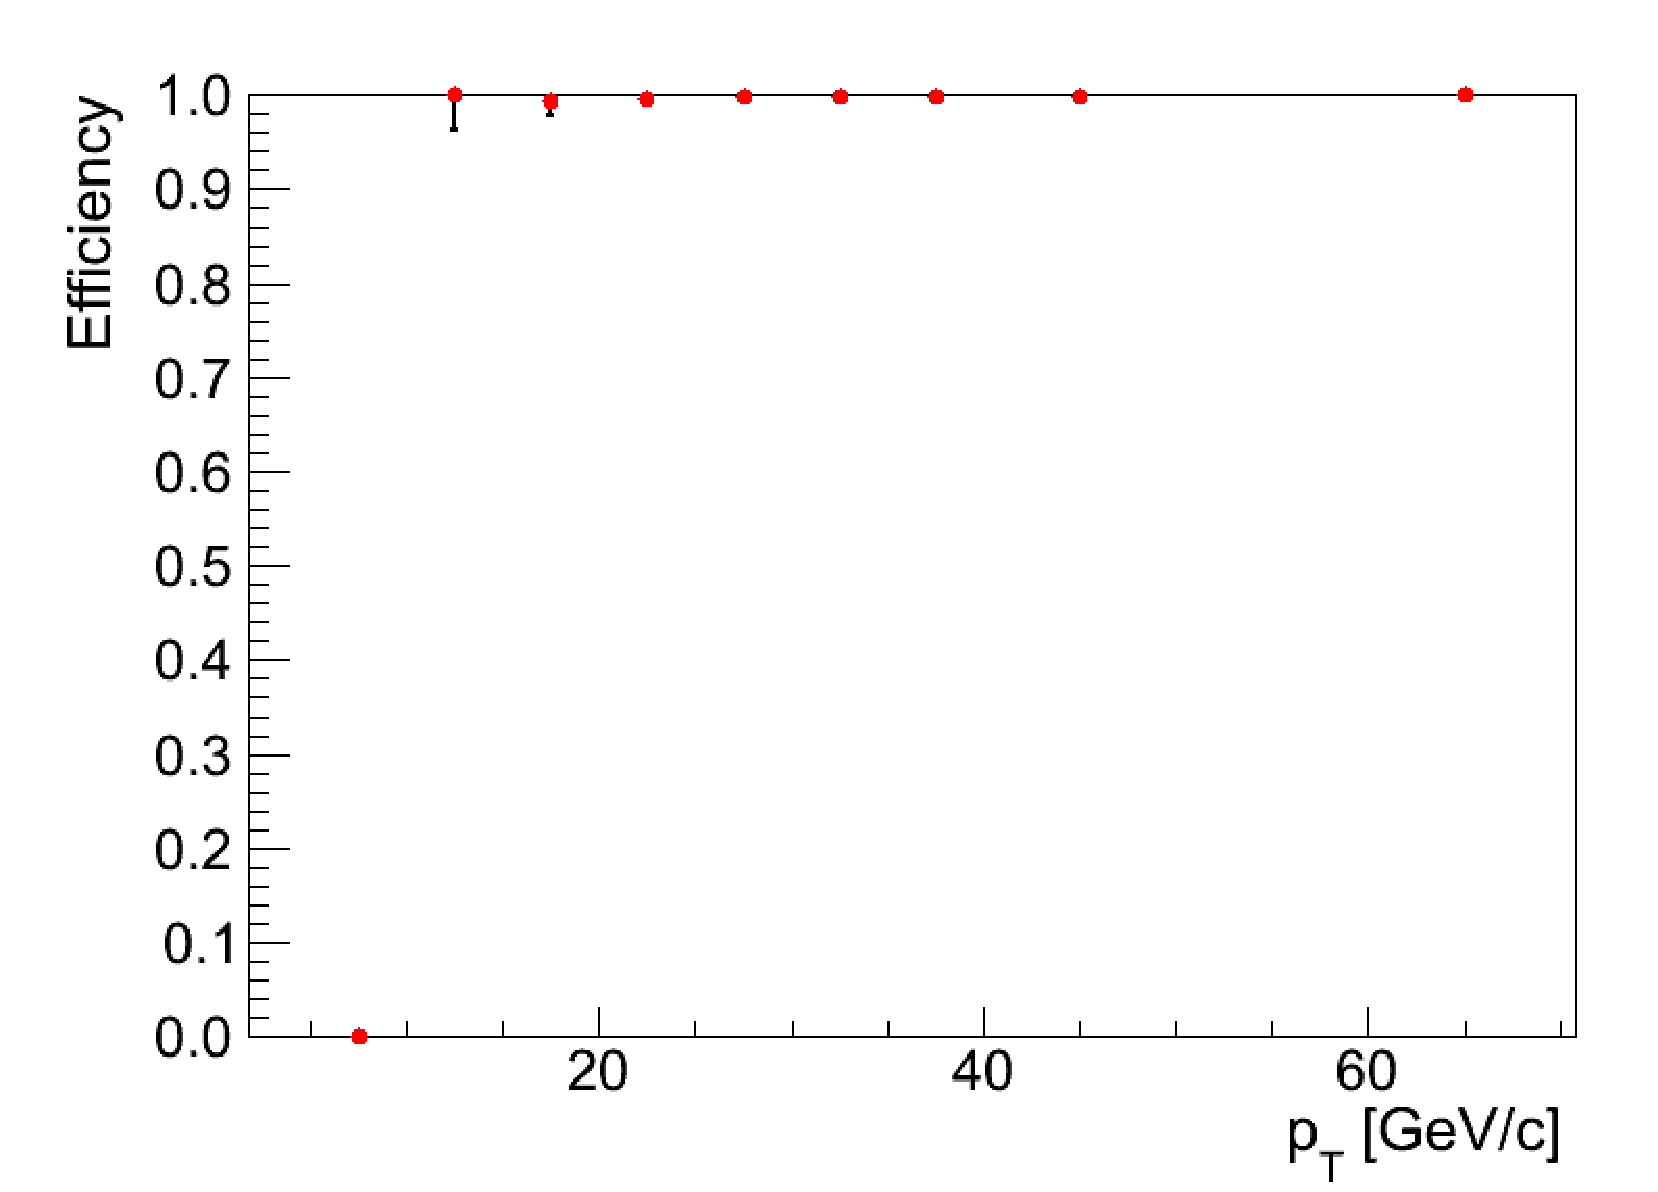
\includegraphics[width=0.48\textwidth]{figures/ElectronTriggerEffVsPt_Ele17Ele8.pdf}
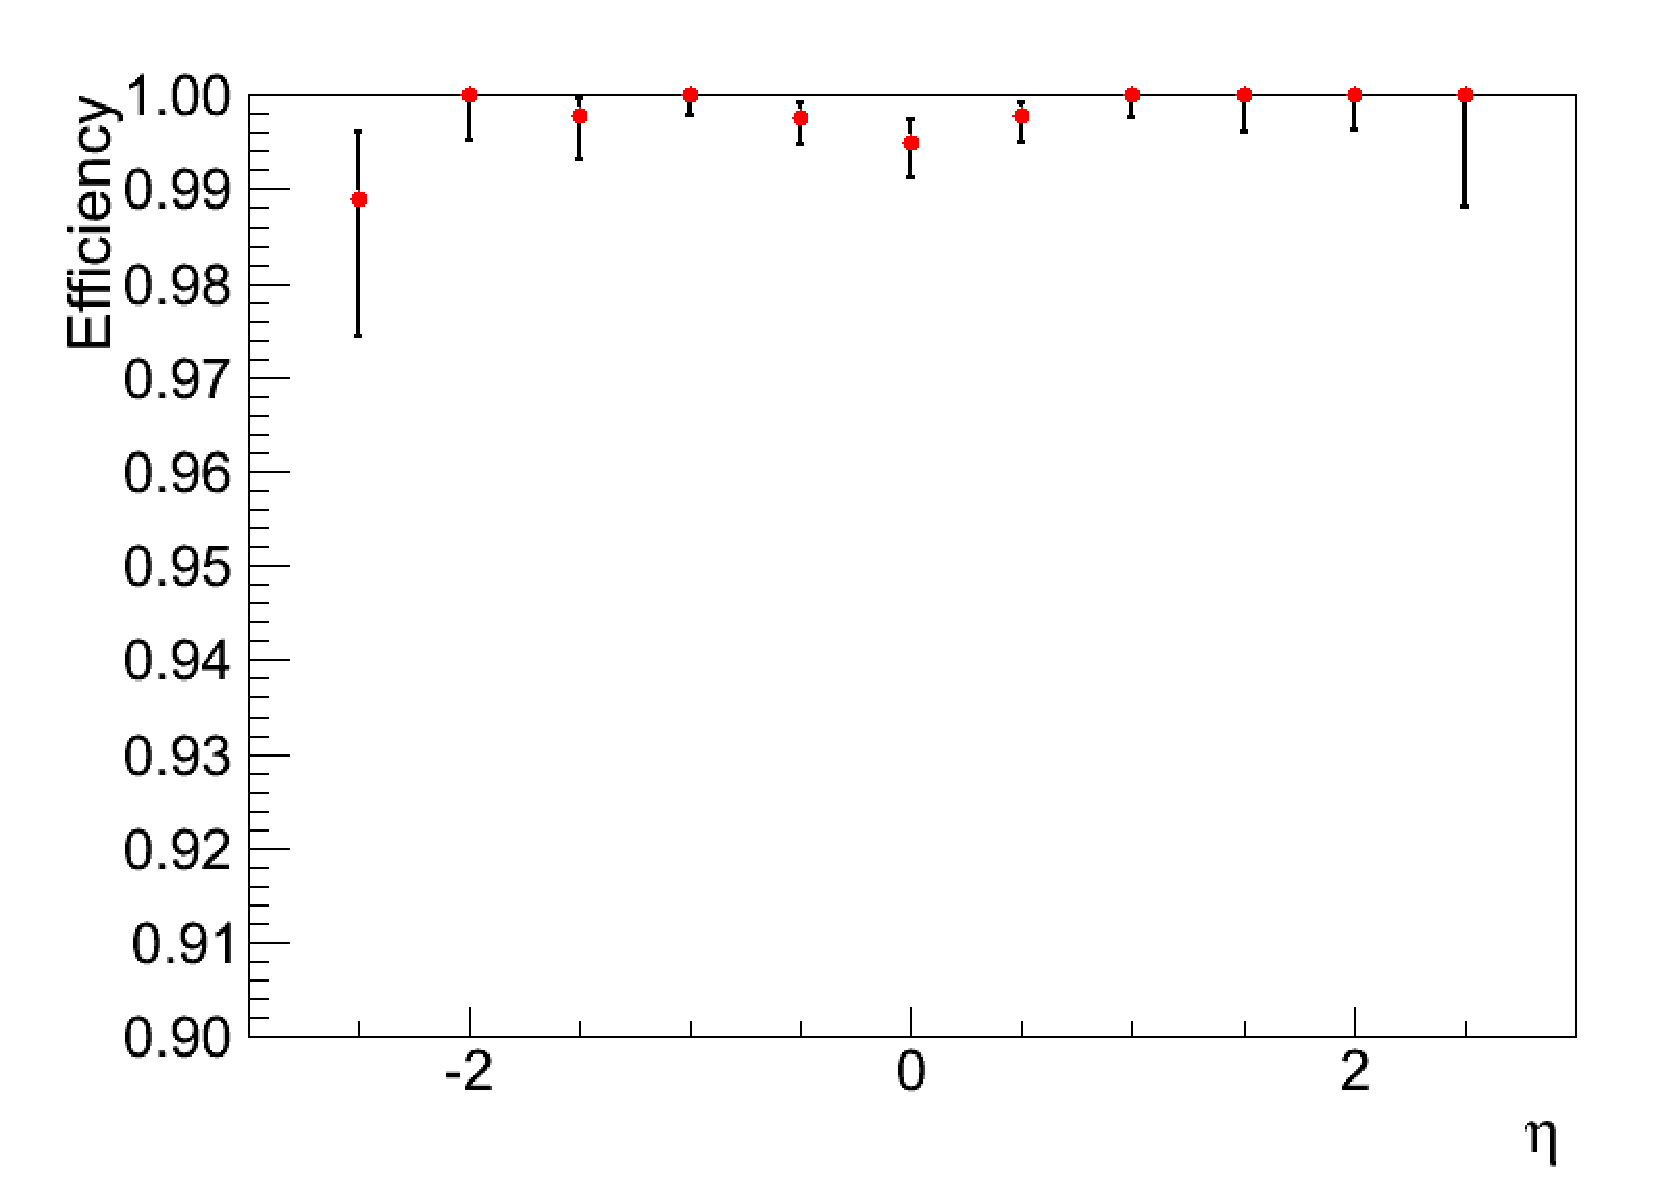
\includegraphics[width=0.48\textwidth]{figures/ElectronTriggerEffVsEta_Ele17Ele8.pdf}
\end{center}
\caption{Efficiency for the unseeded leg of the double electron trigger as a function of $p_{T}$ (a) and $\eta$ (b).}
\label{fig:Ele17Ele8TriggerEfficiencyUnseededLeg}
\end{figure}

\begin{table}[!ht]
\begin{center}
\begin{tabular}{c|c|c} \hline
              & Barrel ( $|\eta|<1.5$ )  & Endcap ( $|\eta|>1.5$ )  \\  \hline
\hline
Seeded Leg 20$<p_{T}<$   & 0.9931 + 0.0012 - 0.0014 & 0.9942 + 0.0019 - 0.0026 \\ \hline
Unseeded Leg 10$<p_{T}<$15 & 1.0 + 0.0 - 0.07 & 1.0 + 0.0 - 0.08                 \\ \hline
Unseeded Leg 15$<p_{T}<$20 & 1.0 + 0.0 - 0.02 & 0.985 + 0.012 - 0.033            \\ \hline
Unseeded Leg 20$<p_{T}<$   & 0.9981 + 0.0006 - 0.0009 & 0.9993 + 0.0005 - 0.0015 \\
\hline
\end{tabular}
\caption{Efficiency for the seeded leg of the double electron trigger 
separately in bins of $p_{T}$ for the barrel and endcap.
\label{tab:eff_double_ele}}
\end{center}
\end{table}

%%%%%% single
The per electron efficiency for the
single electron trigger is shown in Figure \ref{fig:Ele27Efficiency} and summarized
in Table \ref{tab:Ele27Efficiency}. 

\begin{figure}[!ht]
\begin{center}
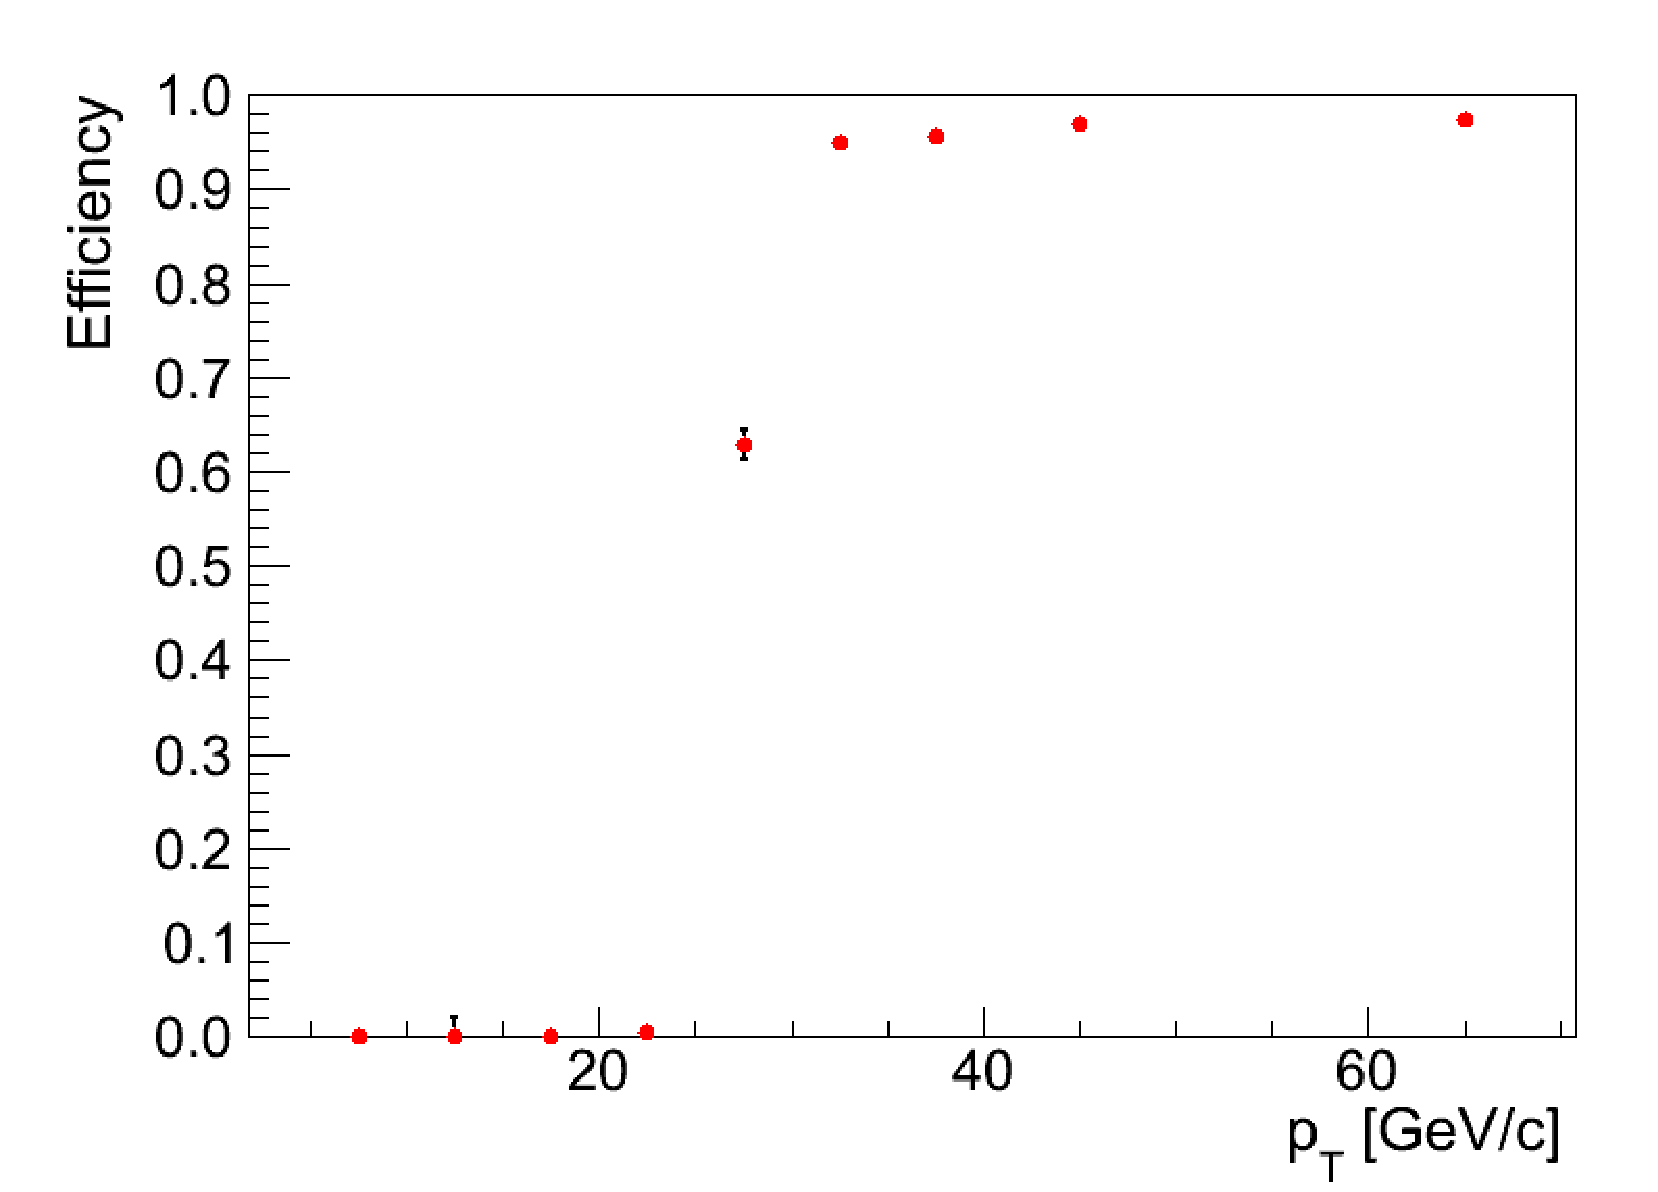
\includegraphics[width=0.48\textwidth]{figures/ElectronTriggerEffVsPt_Ele27Tight.pdf}
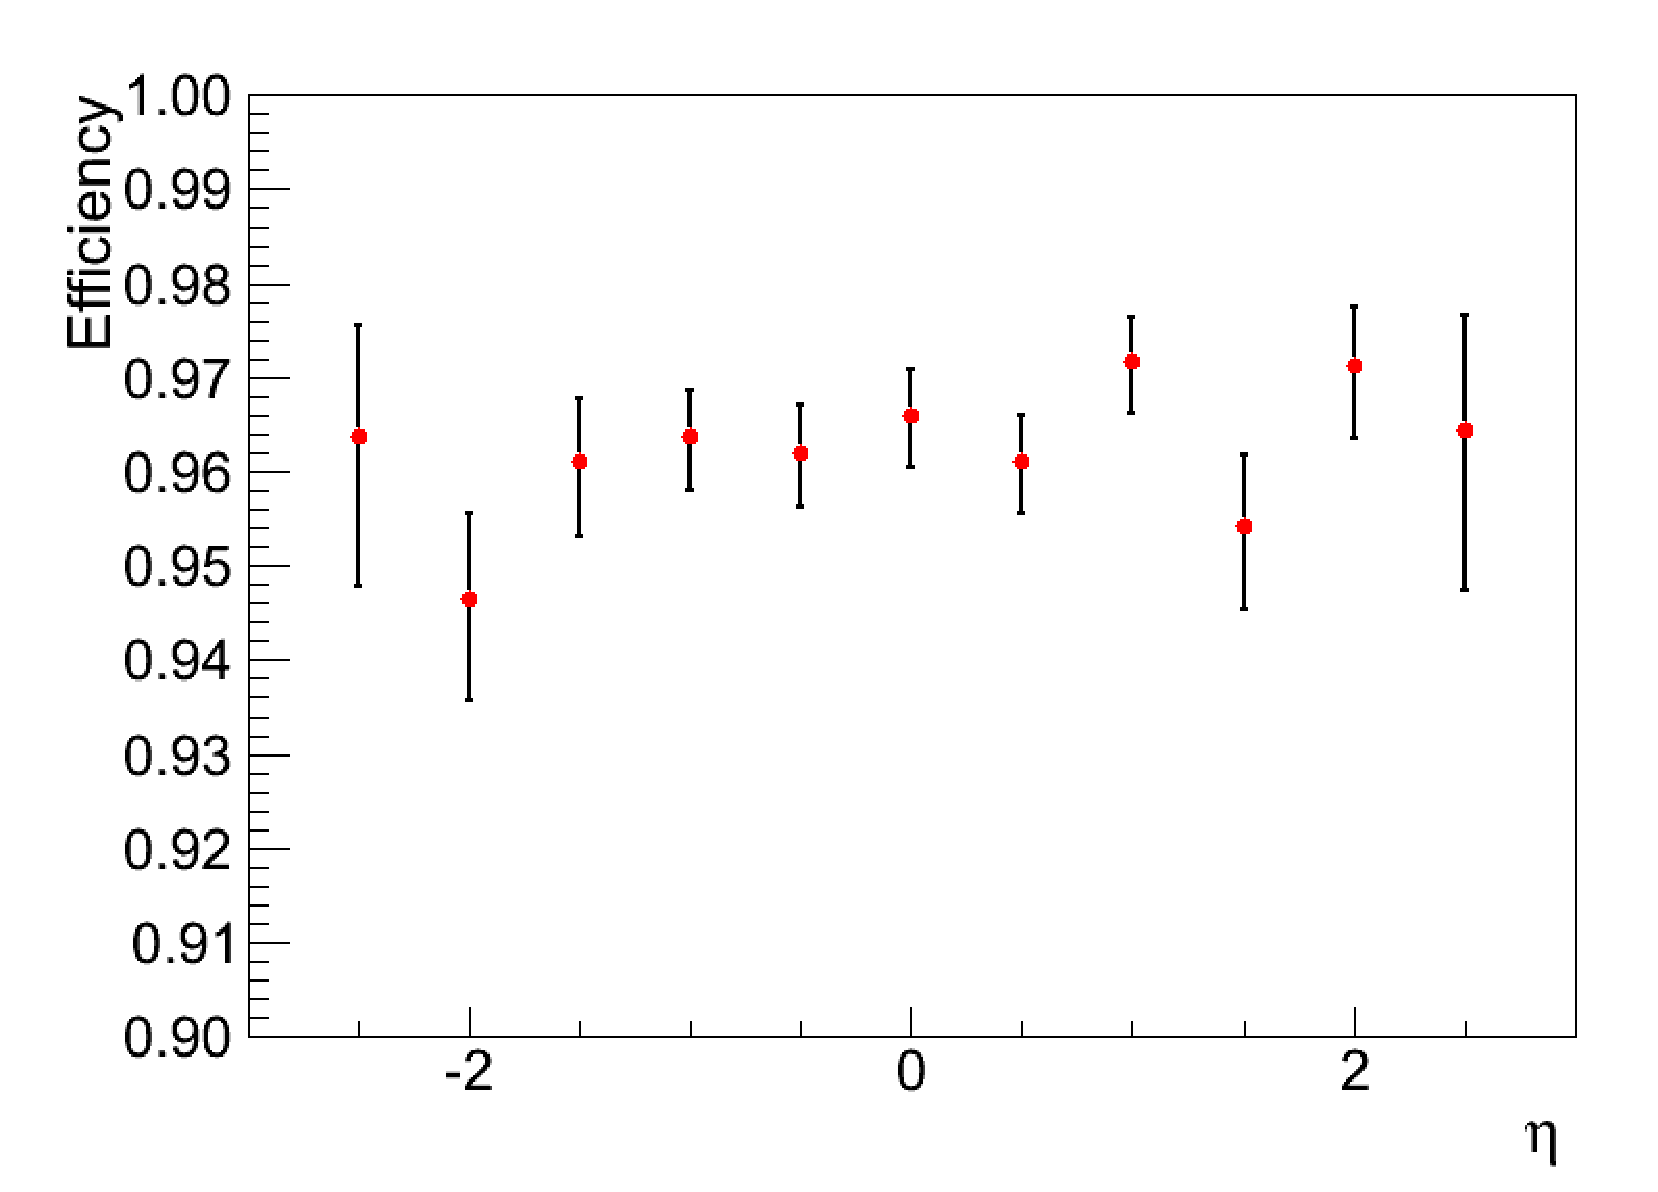
\includegraphics[width=0.48\textwidth]{figures/ElectronTriggerEffVsEta_Ele27Tight.pdf}
\end{center}
\caption{The single leg efficiency of the single electron trigger as a function of $p_{T}$ (a) and $\eta$ (b).}
\label{fig:Ele27Efficiency}
\end{figure}

\begin{table}[!ht]
\begin{center}
\begin{tabular}{c|c|c} \hline
              & Barrel ( $|\eta|<1.5$ )  & Endcap ( $|\eta|>1.5$ )  \\  \hline
\hline
30$<p_{T}<$   & 0.964 + 0.002 - 0.002 & 0.958 + 0.004 - 0.004 \\
\hline
\end{tabular}
\caption{The single leg efficiency of the single electron trigger 
separately in bins of $p_{T}$ for the barrel and endcap.
\label{tab:Ele27Efficiency}}
\end{center}
\end{table}

%
%
%
\subsubsection{Muon triggers}
The double muon trigger requires both legs to be seeded at Level-1.
The per muon efficiency for the double trigger is 
summarized in Table \ref{tab:eff_double_mu}. 


\begin{table}[!ht]
\begin{center}
\begin{tabular}{c|c|c} \hline
              & Barrel ( $|\eta|<1.5$ )  & Endcap ( $|\eta|>1.5$ )  \\  \hline
\hline
20$<p_{T}<$   & XXX$\pm$YYY & XXX$\pm$YYY \\
\hline
\end{tabular}
\caption{Per muon efficiency for HLT\_DoubleMuXXX.}
\label{tab:eff_double_mu}
\end{center}
\end{table}


%% DoubleMu7 Express : 
%% Pt10To15:
%% Barrel Eff : 25/26 = 0.961538 + 0.0318235 - 0.0828584
%% Endcap Eff : 19/20 = 0.95 + 0.0413792 - 0.105642

%% Pt15To20:
%% Barrel Eff : 81/83 = 0.975904 + 0.015537 - 0.0308607
%% Endcap Eff : 51/54 = 0.944444 + 0.0300568 - 0.051037

%% Pt20ToInf:
%% Barrel Eff : 5012/5247 = 0.955213 + 0.00285777 - 0.00303673
%% Endcap Eff : 1906/2044 = 0.932485 + 0.0055673 - 0.00600819

%% DoubleMu7 Prompt Reco : 
%% Pt10To15:
%% Barrel Eff : 33/35 = 0.942857 + 0.0367943 - 0.0703594
%% Endcap Eff : 40/43 = 0.930233 + 0.0376956 - 0.0631583

%% Pt15To20:
%% Barrel Eff : 107/108 = 0.990741 + 0.00765718 - 0.0209429
%% Endcap Eff : 82/83 = 0.987952 + 0.00996406 - 0.0271254

%% Pt20ToInf:
%% Barrel Eff : 5471/5666 = 0.965584 + 0.00242228 - 0.00259228
%% Endcap Eff : 2085/2181 = 0.955983 + 0.00439809 - 0.00483715


%% SingleMu24 Express:
%% Pt20ToInf:
%% Barrel Eff : 6345/6815 = 0.931034 + 0.00307405 - 0.00320332
%% Endcap Eff : 1412/1637 = 0.862553 + 0.00857366 - 0.00903148

%% SingleMu24 PromptReco
%% Pt20ToInf:
%% Barrel Eff : 6713/7233 = 0.928107 + 0.00304181 - 0.00316265
%% Endcap Eff : 1436/1665 = 0.862462 + 0.0085031 - 0.00895298



